\section{Labeled Transition System}
\label{ss:ltstype}

As a simple example of using ITS, let us LTS semantics as an elementary ITS type.
%To have a fully working model definition, we still need to define an elementary type.
We use here a labeled transition system as elementary brick, adapted to the ITS type contract.

\begin{definition}
\label{def:ltstype}
An elementary Labeled Transition System (LTS) is a tuple \\
$LTS = \tuple{N,N_0,L,E,V}$:
\begin{itemize}
\item $N$ is a finite set of nodes;
\item $N_0 \subseteq N$ is a subset of designated initial states;
\item $L$ is a finite set of labels for edges, partitioned into $L_\labloc$ that represents ``local'' labels and $L_\bot$ that contains other labels;
\item $E \subseteq N \times L \times N$ is a set of labeled edges;
\end{itemize}
\end{definition}

The ITS type which corresponds to an elementary LTS, is defined as:
\begin{itemize}
\item $S = N$
%\item $\istate{} = N_0$
\item $A = L_\bot$
\item $\locals: S \mapsto 2^S$ is defined as $n' \in \mathit{Locals}(n)$ iff $\exists l \in L_\labloc$, $\tuple{n,l,n'} \in E$;
\item $\succs{}: S \times  \lang{A}  \mapsto 2^S: \forall n,n' \in S, \forall w= a_1\cdot\ldots\cdot a_m \in \lang{A}, n' \in \succs{}(n,w)$ iff
$\exists n_0,\ldots, n_m \in N$ such that $n_0 = n$ and $n_m = n'$, and $\forall j, 0 \leq j < m, \tuple{n_j,a_{j+1},n_{j+1}} \in E$

$\succs{}(n,\tau) = \emptyset$ if $\tau$ contains more than one transition label.
Else, when $\tau= \{l\}$, $\forall n,n' \in S, n' \in \succs{}(n,\{l\})$ iff $\tuple{n,l,n'} \in E$.
\end{itemize}

As an example, Fig.~\ref{fig:lts} represents an implementation of the Process type introduced earlier (Fig. \ref{fig:types}) using an LTS.
\begin{figure}[htbp]
\center
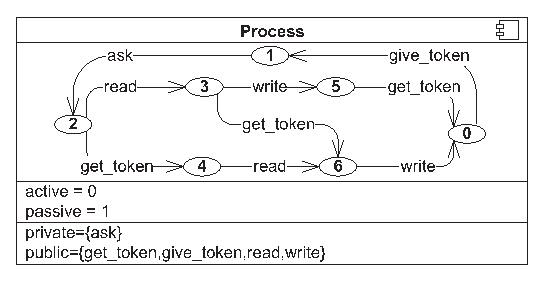
\includegraphics[scale=0.8]{lts-fig.eps}
\caption{An LTS representing an implementation of the Process type in the round robin protocol. \label{fig:lts}}
\end{figure}

\emph{Encoding:} we index the states of LTS, and use an SDD with a single
variable of integer domain reflecting the current state. The transition
relation is easily realized using a precomputed transition function $f:S
\times L \mapsto 2^S$ such that $f(n,l) = \{ n' \mid \tuple{n,l,n'} \in E \}$.
Furthermore, for any set $s \subseteq S$ we define the set $\mathit{priv}(s) = \bigcup_{x
\in s} \bigcup_{l \in L \land V(l)=private} f(x,l)$.

$\mathit{Locals}$ and \succs{} are defined using inductive homomorphisms.
Note that as we have a single variable in the encoding these homomorphisms do not need to propagate.
\succs{} is defined below when the argument $\tau \in \bag(T)$ contains a single transition label $l$.
Otherwise it returns the terminal $0$.

$
\begin{array}{ll}
\left\{
\begin{array}{lcl}
\mathit{Locals} (\omega,s) & = & e \fireseq{\mathit{priv}(s)} \id{} \\
\mathit{Locals} (1) &=& 1
\end{array}
\right.
&
\left\{
\begin{array}{lcl}
\succs (l)(\omega,s)& = &e \fireseq{\bigcup_{x \in s} f(x,l)} \id{} \\
\succs (l)(1) &= &1
\end{array}
\right.
\end{array}
$

